\documentclass[twoside]{book}

% Packages required by doxygen
\usepackage{fixltx2e}
\usepackage{calc}
\usepackage{doxygen}
\usepackage[export]{adjustbox} % also loads graphicx
\usepackage{graphicx}
\usepackage[utf8]{inputenc}
\usepackage{makeidx}
\usepackage{multicol}
\usepackage{multirow}
\PassOptionsToPackage{warn}{textcomp}
\usepackage{textcomp}
\usepackage[nointegrals]{wasysym}
\usepackage[table]{xcolor}

% Font selection
\usepackage[T1]{fontenc}
\usepackage[scaled=.90]{helvet}
\usepackage{courier}
\usepackage{amssymb}
\usepackage{sectsty}
\renewcommand{\familydefault}{\sfdefault}
\allsectionsfont{%
  \fontseries{bc}\selectfont%
  \color{darkgray}%
}
\renewcommand{\DoxyLabelFont}{%
  \fontseries{bc}\selectfont%
  \color{darkgray}%
}
\newcommand{\+}{\discretionary{\mbox{\scriptsize$\hookleftarrow$}}{}{}}

% Page & text layout
\usepackage{geometry}
\geometry{%
  a4paper,%
  top=2.5cm,%
  bottom=2.5cm,%
  left=2.5cm,%
  right=2.5cm%
}
\tolerance=750
\hfuzz=15pt
\hbadness=750
\setlength{\emergencystretch}{15pt}
\setlength{\parindent}{0cm}
\setlength{\parskip}{0.2cm}
\makeatletter
\renewcommand{\paragraph}{%
  \@startsection{paragraph}{4}{0ex}{-1.0ex}{1.0ex}{%
    \normalfont\normalsize\bfseries\SS@parafont%
  }%
}
\renewcommand{\subparagraph}{%
  \@startsection{subparagraph}{5}{0ex}{-1.0ex}{1.0ex}{%
    \normalfont\normalsize\bfseries\SS@subparafont%
  }%
}
\makeatother

% Headers & footers
\usepackage{fancyhdr}
\pagestyle{fancyplain}
\fancyhead[LE]{\fancyplain{}{\bfseries\thepage}}
\fancyhead[CE]{\fancyplain{}{}}
\fancyhead[RE]{\fancyplain{}{\bfseries\leftmark}}
\fancyhead[LO]{\fancyplain{}{\bfseries\rightmark}}
\fancyhead[CO]{\fancyplain{}{}}
\fancyhead[RO]{\fancyplain{}{\bfseries\thepage}}
\fancyfoot[LE]{\fancyplain{}{}}
\fancyfoot[CE]{\fancyplain{}{}}
\fancyfoot[RE]{\fancyplain{}{\bfseries\scriptsize Generated on Tue Apr 26 2016 14\+:30\+:48 for My Project by Doxygen }}
\fancyfoot[LO]{\fancyplain{}{\bfseries\scriptsize Generated on Tue Apr 26 2016 14\+:30\+:48 for My Project by Doxygen }}
\fancyfoot[CO]{\fancyplain{}{}}
\fancyfoot[RO]{\fancyplain{}{}}
\renewcommand{\footrulewidth}{0.4pt}
\renewcommand{\chaptermark}[1]{%
  \markboth{#1}{}%
}
\renewcommand{\sectionmark}[1]{%
  \markright{\thesection\ #1}%
}

% Indices & bibliography
\usepackage{natbib}
\usepackage[titles]{tocloft}
\setcounter{tocdepth}{3}
\setcounter{secnumdepth}{5}
\makeindex

% Hyperlinks (required, but should be loaded last)
\usepackage{ifpdf}
\ifpdf
  \usepackage[pdftex,pagebackref=true]{hyperref}
\else
  \usepackage[ps2pdf,pagebackref=true]{hyperref}
\fi
\hypersetup{%
  colorlinks=true,%
  linkcolor=blue,%
  citecolor=blue,%
  unicode%
}

% Custom commands
\newcommand{\clearemptydoublepage}{%
  \newpage{\pagestyle{empty}\cleardoublepage}%
}


%===== C O N T E N T S =====

\begin{document}

% Titlepage & ToC
\hypersetup{pageanchor=false,
             bookmarks=true,
             bookmarksnumbered=true,
             pdfencoding=unicode
            }
\pagenumbering{roman}
\begin{titlepage}
\vspace*{7cm}
\begin{center}%
{\Large My Project }\\
\vspace*{1cm}
{\large Generated by Doxygen 1.8.9.1}\\
\vspace*{0.5cm}
{\small Tue Apr 26 2016 14:30:48}\\
\end{center}
\end{titlepage}
\clearemptydoublepage
\tableofcontents
\clearemptydoublepage
\pagenumbering{arabic}
\hypersetup{pageanchor=true}

%--- Begin generated contents ---
\chapter{Hierarchical Index}
\section{Class Hierarchy}
This inheritance list is sorted roughly, but not completely, alphabetically\+:\begin{DoxyCompactList}
\item Form\begin{DoxyCompactList}
\item \contentsline{section}{article.\+forms.\+add\+Form}{\pageref{classarticle_1_1forms_1_1addForm}}{}
\end{DoxyCompactList}
\item Model\begin{DoxyCompactList}
\item \contentsline{section}{article.\+models.\+Article}{\pageref{classarticle_1_1models_1_1Article}}{}
\item \contentsline{section}{article.\+models.\+User}{\pageref{classarticle_1_1models_1_1User}}{}
\end{DoxyCompactList}
\item App\+Config\begin{DoxyCompactList}
\item \contentsline{section}{article.\+apps.\+Article\+Config}{\pageref{classarticle_1_1apps_1_1ArticleConfig}}{}
\end{DoxyCompactList}
\item Test\+Case\begin{DoxyCompactList}
\item \contentsline{section}{article.\+tests.\+Article\+Test\+Case}{\pageref{classarticle_1_1tests_1_1ArticleTestCase}}{}
\item \contentsline{section}{article.\+tests.\+User\+Test\+Case}{\pageref{classarticle_1_1tests_1_1UserTestCase}}{}
\end{DoxyCompactList}
\end{DoxyCompactList}

\chapter{Class Index}
\section{Class List}
Here are the classes, structs, unions and interfaces with brief descriptions\+:\begin{DoxyCompactList}
\item\contentsline{section}{\hyperlink{classarticle_1_1forms_1_1addForm}{article.\+forms.\+add\+Form} }{\pageref{classarticle_1_1forms_1_1addForm}}{}
\item\contentsline{section}{\hyperlink{classarticle_1_1models_1_1Article}{article.\+models.\+Article} }{\pageref{classarticle_1_1models_1_1Article}}{}
\item\contentsline{section}{\hyperlink{classarticle_1_1apps_1_1ArticleConfig}{article.\+apps.\+Article\+Config} }{\pageref{classarticle_1_1apps_1_1ArticleConfig}}{}
\item\contentsline{section}{\hyperlink{classarticle_1_1tests_1_1ArticleTestCase}{article.\+tests.\+Article\+Test\+Case} }{\pageref{classarticle_1_1tests_1_1ArticleTestCase}}{}
\item\contentsline{section}{\hyperlink{classarticle_1_1models_1_1User}{article.\+models.\+User} }{\pageref{classarticle_1_1models_1_1User}}{}
\item\contentsline{section}{\hyperlink{classarticle_1_1tests_1_1UserTestCase}{article.\+tests.\+User\+Test\+Case} }{\pageref{classarticle_1_1tests_1_1UserTestCase}}{}
\end{DoxyCompactList}

\chapter{Class Documentation}
\hypertarget{classarticle_1_1forms_1_1addForm}{}\section{article.\+forms.\+add\+Form Class Reference}
\label{classarticle_1_1forms_1_1addForm}\index{article.\+forms.\+add\+Form@{article.\+forms.\+add\+Form}}


Inheritance diagram for article.\+forms.\+add\+Form\+:
\nopagebreak
\begin{figure}[H]
\begin{center}
\leavevmode
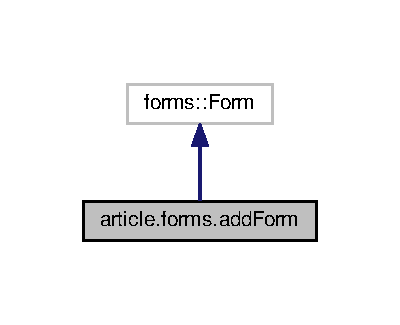
\includegraphics[width=192pt]{classarticle_1_1forms_1_1addForm__inherit__graph}
\end{center}
\end{figure}


Collaboration diagram for article.\+forms.\+add\+Form\+:
\nopagebreak
\begin{figure}[H]
\begin{center}
\leavevmode
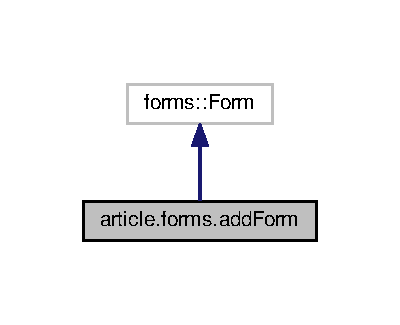
\includegraphics[width=192pt]{classarticle_1_1forms_1_1addForm__coll__graph}
\end{center}
\end{figure}
\subsection*{Static Public Attributes}
\begin{DoxyCompactItemize}
\item 
\hypertarget{classarticle_1_1forms_1_1addForm_a1c672c58060e116ecdc354974c0048cf}{}tuple {\bfseries image} = forms.\+Image\+Field(required=False)\label{classarticle_1_1forms_1_1addForm_a1c672c58060e116ecdc354974c0048cf}

\end{DoxyCompactItemize}


The documentation for this class was generated from the following file\+:\begin{DoxyCompactItemize}
\item 
forms.\+py\end{DoxyCompactItemize}

\hypertarget{classarticle_1_1models_1_1Article}{}\section{article.\+models.\+Article Class Reference}
\label{classarticle_1_1models_1_1Article}\index{article.\+models.\+Article@{article.\+models.\+Article}}


Inheritance diagram for article.\+models.\+Article\+:
\nopagebreak
\begin{figure}[H]
\begin{center}
\leavevmode
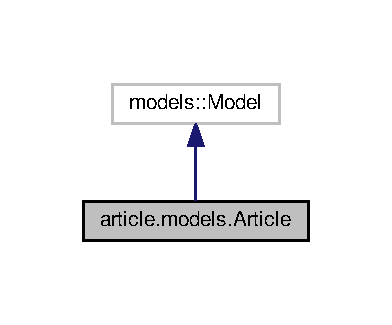
\includegraphics[width=188pt]{classarticle_1_1models_1_1Article__inherit__graph}
\end{center}
\end{figure}


Collaboration diagram for article.\+models.\+Article\+:
\nopagebreak
\begin{figure}[H]
\begin{center}
\leavevmode
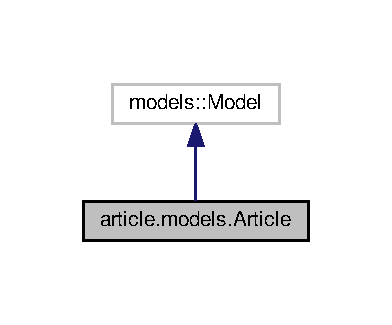
\includegraphics[width=188pt]{classarticle_1_1models_1_1Article__coll__graph}
\end{center}
\end{figure}
\subsection*{Public Member Functions}
\begin{DoxyCompactItemize}
\item 
\hypertarget{classarticle_1_1models_1_1Article_a5ab20899eca1bb6e672c5bde34115f8d}{}def {\bfseries \+\_\+\+\_\+str\+\_\+\+\_\+} (self)\label{classarticle_1_1models_1_1Article_a5ab20899eca1bb6e672c5bde34115f8d}

\end{DoxyCompactItemize}
\subsection*{Static Public Attributes}
\begin{DoxyCompactItemize}
\item 
\hypertarget{classarticle_1_1models_1_1Article_a94ddfc04825577cafc687f5cec3242f0}{}tuple {\bfseries title} = models.\+Char\+Field(max\+\_\+length = 100)\label{classarticle_1_1models_1_1Article_a94ddfc04825577cafc687f5cec3242f0}

\item 
\hypertarget{classarticle_1_1models_1_1Article_af63605372e5e04d50afbcf885a322a83}{}tuple {\bfseries category} = models.\+Char\+Field(max\+\_\+length = 50,blank=True)\label{classarticle_1_1models_1_1Article_af63605372e5e04d50afbcf885a322a83}

\item 
\hypertarget{classarticle_1_1models_1_1Article_a6d090daa50c903645de2b93db914fc8e}{}tuple {\bfseries date\+\_\+time} = models.\+Date\+Time\+Field(default = timezone.\+now())\label{classarticle_1_1models_1_1Article_a6d090daa50c903645de2b93db914fc8e}

\item 
\hypertarget{classarticle_1_1models_1_1Article_a88570c13409c321dc73630797411b99d}{}tuple {\bfseries content} = models.\+Text\+Field(blank =True,null=True)\label{classarticle_1_1models_1_1Article_a88570c13409c321dc73630797411b99d}

\item 
\hypertarget{classarticle_1_1models_1_1Article_af26f156302a0b4e467b8af91f493b095}{}tuple {\bfseries username} = models.\+Char\+Field(max\+\_\+length = 100,default=\textquotesingle{}S\+O\+M\+E S\+T\+R\+I\+N\+G\textquotesingle{})\label{classarticle_1_1models_1_1Article_af26f156302a0b4e467b8af91f493b095}

\item 
\hypertarget{classarticle_1_1models_1_1Article_a85b36fb0f467c7c7d9416def1e1cb601}{}tuple {\bfseries image} = models.\+Image\+Field(upload\+\_\+to=\textquotesingle{}photos\textquotesingle{}, blank=True,null=True)\label{classarticle_1_1models_1_1Article_a85b36fb0f467c7c7d9416def1e1cb601}

\end{DoxyCompactItemize}


The documentation for this class was generated from the following file\+:\begin{DoxyCompactItemize}
\item 
models.\+py\end{DoxyCompactItemize}

\hypertarget{classarticle_1_1apps_1_1ArticleConfig}{}\section{article.\+apps.\+Article\+Config Class Reference}
\label{classarticle_1_1apps_1_1ArticleConfig}\index{article.\+apps.\+Article\+Config@{article.\+apps.\+Article\+Config}}


Inheritance diagram for article.\+apps.\+Article\+Config\+:
\nopagebreak
\begin{figure}[H]
\begin{center}
\leavevmode
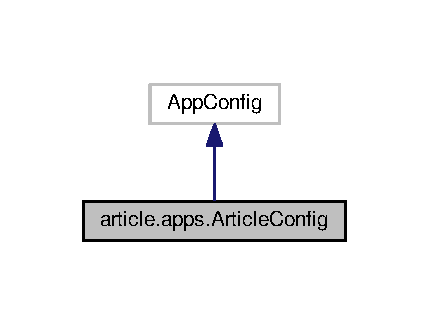
\includegraphics[width=206pt]{classarticle_1_1apps_1_1ArticleConfig__inherit__graph}
\end{center}
\end{figure}


Collaboration diagram for article.\+apps.\+Article\+Config\+:
\nopagebreak
\begin{figure}[H]
\begin{center}
\leavevmode
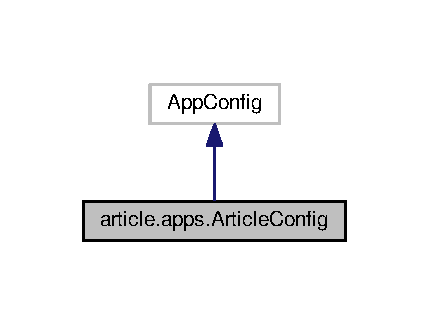
\includegraphics[width=206pt]{classarticle_1_1apps_1_1ArticleConfig__coll__graph}
\end{center}
\end{figure}
\subsection*{Static Public Attributes}
\begin{DoxyCompactItemize}
\item 
\hypertarget{classarticle_1_1apps_1_1ArticleConfig_ade0b2cad93d9873fde99a9e3ed0e3190}{}string {\bfseries name} = \textquotesingle{}article\textquotesingle{}\label{classarticle_1_1apps_1_1ArticleConfig_ade0b2cad93d9873fde99a9e3ed0e3190}

\end{DoxyCompactItemize}


The documentation for this class was generated from the following file\+:\begin{DoxyCompactItemize}
\item 
apps.\+py\end{DoxyCompactItemize}

\hypertarget{classarticle_1_1tests_1_1ArticleTestCase}{}\section{article.\+tests.\+Article\+Test\+Case Class Reference}
\label{classarticle_1_1tests_1_1ArticleTestCase}\index{article.\+tests.\+Article\+Test\+Case@{article.\+tests.\+Article\+Test\+Case}}


Inheritance diagram for article.\+tests.\+Article\+Test\+Case\+:
\nopagebreak
\begin{figure}[H]
\begin{center}
\leavevmode
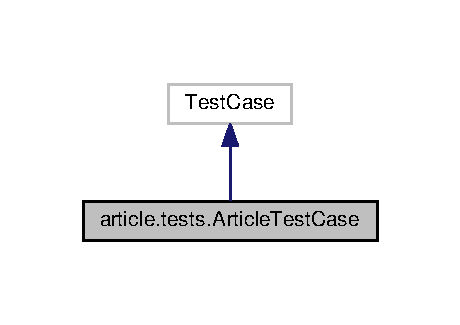
\includegraphics[width=221pt]{classarticle_1_1tests_1_1ArticleTestCase__inherit__graph}
\end{center}
\end{figure}


Collaboration diagram for article.\+tests.\+Article\+Test\+Case\+:
\nopagebreak
\begin{figure}[H]
\begin{center}
\leavevmode
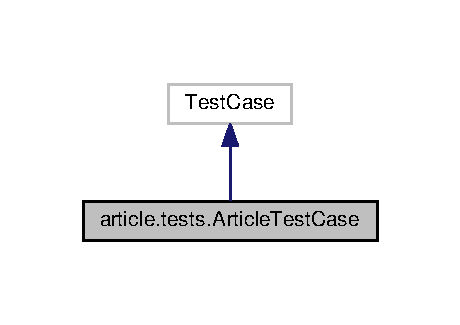
\includegraphics[width=221pt]{classarticle_1_1tests_1_1ArticleTestCase__coll__graph}
\end{center}
\end{figure}
\subsection*{Public Member Functions}
\begin{DoxyCompactItemize}
\item 
\hypertarget{classarticle_1_1tests_1_1ArticleTestCase_a2b468a7bb6ccf7dc9ce29d8b5bf664ab}{}def {\bfseries set\+Up} (self)\label{classarticle_1_1tests_1_1ArticleTestCase_a2b468a7bb6ccf7dc9ce29d8b5bf664ab}

\item 
\hypertarget{classarticle_1_1tests_1_1ArticleTestCase_a03d845b8569bdac1c0e6c2051f7c0129}{}def {\bfseries test\+\_\+\+Article} (self)\label{classarticle_1_1tests_1_1ArticleTestCase_a03d845b8569bdac1c0e6c2051f7c0129}

\end{DoxyCompactItemize}


The documentation for this class was generated from the following file\+:\begin{DoxyCompactItemize}
\item 
tests.\+py\end{DoxyCompactItemize}

\hypertarget{classarticle_1_1models_1_1User}{}\section{article.\+models.\+User Class Reference}
\label{classarticle_1_1models_1_1User}\index{article.\+models.\+User@{article.\+models.\+User}}


Inheritance diagram for article.\+models.\+User\+:
\nopagebreak
\begin{figure}[H]
\begin{center}
\leavevmode
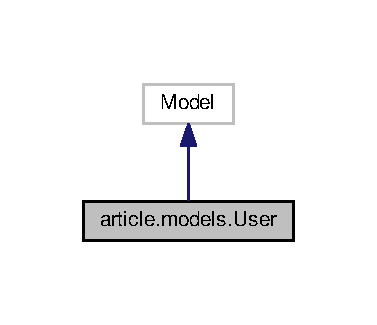
\includegraphics[width=181pt]{classarticle_1_1models_1_1User__inherit__graph}
\end{center}
\end{figure}


Collaboration diagram for article.\+models.\+User\+:
\nopagebreak
\begin{figure}[H]
\begin{center}
\leavevmode
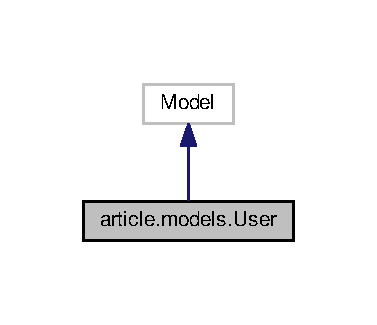
\includegraphics[width=181pt]{classarticle_1_1models_1_1User__coll__graph}
\end{center}
\end{figure}
\subsection*{Public Member Functions}
\begin{DoxyCompactItemize}
\item 
\hypertarget{classarticle_1_1models_1_1User_aea047e9228c3645d2b1a338bcb5cefc5}{}def {\bfseries \+\_\+\+\_\+str\+\_\+\+\_\+} (self)\label{classarticle_1_1models_1_1User_aea047e9228c3645d2b1a338bcb5cefc5}

\end{DoxyCompactItemize}
\subsection*{Static Public Attributes}
\begin{DoxyCompactItemize}
\item 
\hypertarget{classarticle_1_1models_1_1User_a76f3a104d8dabd110be8cc59b044a442}{}tuple {\bfseries username} = models.\+Char\+Field(max\+\_\+length = 100,default=\textquotesingle{}S\+O\+M\+E S\+T\+R\+I\+N\+G\textquotesingle{})\label{classarticle_1_1models_1_1User_a76f3a104d8dabd110be8cc59b044a442}

\item 
\hypertarget{classarticle_1_1models_1_1User_aeb929515f62ba5156fc9230e8fad0493}{}tuple {\bfseries email} = models.\+Email\+Field(max\+\_\+length = 254)\label{classarticle_1_1models_1_1User_aeb929515f62ba5156fc9230e8fad0493}

\item 
\hypertarget{classarticle_1_1models_1_1User_ad838cb6e13774bb438a8c436fabd657e}{}tuple {\bfseries password} = models.\+Char\+Field(max\+\_\+length=100)\label{classarticle_1_1models_1_1User_ad838cb6e13774bb438a8c436fabd657e}

\item 
\hypertarget{classarticle_1_1models_1_1User_abc7ee742586e7b3cfd65cecee79b83b5}{}tuple {\bfseries user\+\_\+id} = models.\+Big\+Integer\+Field(default = -\/1)\label{classarticle_1_1models_1_1User_abc7ee742586e7b3cfd65cecee79b83b5}

\end{DoxyCompactItemize}


The documentation for this class was generated from the following file\+:\begin{DoxyCompactItemize}
\item 
models.\+py\end{DoxyCompactItemize}

\hypertarget{classarticle_1_1tests_1_1UserTestCase}{}\section{article.\+tests.\+User\+Test\+Case Class Reference}
\label{classarticle_1_1tests_1_1UserTestCase}\index{article.\+tests.\+User\+Test\+Case@{article.\+tests.\+User\+Test\+Case}}


Inheritance diagram for article.\+tests.\+User\+Test\+Case\+:
\nopagebreak
\begin{figure}[H]
\begin{center}
\leavevmode
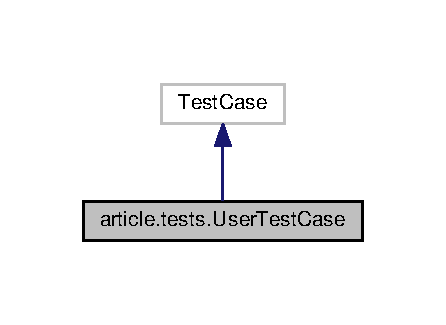
\includegraphics[width=214pt]{classarticle_1_1tests_1_1UserTestCase__inherit__graph}
\end{center}
\end{figure}


Collaboration diagram for article.\+tests.\+User\+Test\+Case\+:
\nopagebreak
\begin{figure}[H]
\begin{center}
\leavevmode
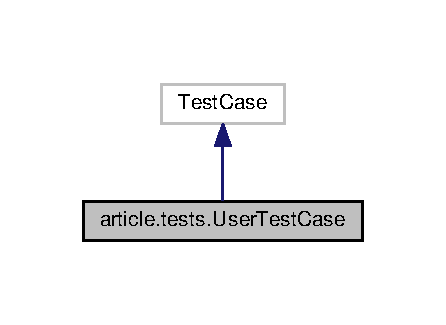
\includegraphics[width=214pt]{classarticle_1_1tests_1_1UserTestCase__coll__graph}
\end{center}
\end{figure}
\subsection*{Public Member Functions}
\begin{DoxyCompactItemize}
\item 
\hypertarget{classarticle_1_1tests_1_1UserTestCase_a54377c8aa9dfd39345985593c42e4fa0}{}def {\bfseries set\+Up} (self)\label{classarticle_1_1tests_1_1UserTestCase_a54377c8aa9dfd39345985593c42e4fa0}

\item 
\hypertarget{classarticle_1_1tests_1_1UserTestCase_a0f6b99c4291fc4880d41a2013c083530}{}def {\bfseries test\+\_\+\+User} (self)\label{classarticle_1_1tests_1_1UserTestCase_a0f6b99c4291fc4880d41a2013c083530}

\end{DoxyCompactItemize}


The documentation for this class was generated from the following file\+:\begin{DoxyCompactItemize}
\item 
tests.\+py\end{DoxyCompactItemize}

%--- End generated contents ---

% Index
\backmatter
\newpage
\phantomsection
\clearemptydoublepage
\addcontentsline{toc}{chapter}{Index}
\printindex

\end{document}
